\documentclass[a4paper]{article}\usepackage[]{graphicx}\usepackage[]{color}
%% maxwidth is the original width if it is less than linewidth
%% otherwise use linewidth (to make sure the graphics do not exceed the margin)
\makeatletter
\def\maxwidth{ %
  \ifdim\Gin@nat@width>\linewidth
    \linewidth
  \else
    \Gin@nat@width
  \fi
}
\makeatother

\definecolor{fgcolor}{rgb}{0.345, 0.345, 0.345}
\newcommand{\hlnum}[1]{\textcolor[rgb]{0.686,0.059,0.569}{#1}}%
\newcommand{\hlstr}[1]{\textcolor[rgb]{0.192,0.494,0.8}{#1}}%
\newcommand{\hlcom}[1]{\textcolor[rgb]{0.678,0.584,0.686}{\textit{#1}}}%
\newcommand{\hlopt}[1]{\textcolor[rgb]{0,0,0}{#1}}%
\newcommand{\hlstd}[1]{\textcolor[rgb]{0.345,0.345,0.345}{#1}}%
\newcommand{\hlkwa}[1]{\textcolor[rgb]{0.161,0.373,0.58}{\textbf{#1}}}%
\newcommand{\hlkwb}[1]{\textcolor[rgb]{0.69,0.353,0.396}{#1}}%
\newcommand{\hlkwc}[1]{\textcolor[rgb]{0.333,0.667,0.333}{#1}}%
\newcommand{\hlkwd}[1]{\textcolor[rgb]{0.737,0.353,0.396}{\textbf{#1}}}%

\usepackage{framed}
\makeatletter
\newenvironment{kframe}{%
 \def\at@end@of@kframe{}%
 \ifinner\ifhmode%
  \def\at@end@of@kframe{\end{minipage}}%
  \begin{minipage}{\columnwidth}%
 \fi\fi%
 \def\FrameCommand##1{\hskip\@totalleftmargin \hskip-\fboxsep
 \colorbox{shadecolor}{##1}\hskip-\fboxsep
     % There is no \\@totalrightmargin, so:
     \hskip-\linewidth \hskip-\@totalleftmargin \hskip\columnwidth}%
 \MakeFramed {\advance\hsize-\width
   \@totalleftmargin\z@ \linewidth\hsize
   \@setminipage}}%
 {\par\unskip\endMakeFramed%
 \at@end@of@kframe}
\makeatother

\definecolor{shadecolor}{rgb}{.97, .97, .97}
\definecolor{messagecolor}{rgb}{0, 0, 0}
\definecolor{warningcolor}{rgb}{1, 0, 1}
\definecolor{errorcolor}{rgb}{1, 0, 0}
\newenvironment{knitrout}{}{} % an empty environment to be redefined in TeX

\usepackage{alltt}

\usepackage{amsmath}
\usepackage{amssymb}
\usepackage{parskip}
\usepackage{natbib}
\bibpunct{(}{)}{;}{a}{}{,}
\usepackage{hyperref}
\usepackage[margin=1in]{geometry}
\usepackage[labelfont={bf}, margin=0.5cm]{caption}

%\VignetteIndexEntry{Examples using SimLongi}
%\VignetteDepends{SimLongi}
%\VignetteKeywords{linear mixed-effects model, multiple contrast test, simultaneous confidence interval}

\title{Simultaneous inference in longitudinal settings: Examples using package \texttt{SimLongi}}
\date{\today}
\author{Philip Pallmann}
\IfFileExists{upquote.sty}{\usepackage{upquote}}{}

\begin{document}

\maketitle

\tableofcontents

%%%%%%%%%%%%%%%%%%%%%%%%%%%%%%%%%%%%%%%%%%%%%%%%%%%%%%%%%%%%%%%%%%%%%%%%%%%%%%%%%%%%%%%%%%%%%%%%%%%%%%%%%%%%%%%%%%%%%%%%%%%%%%%%%%
%%%%%%%%%%%%%%%%%%%%%%%%%%%%%%%%%%%%%%%%%%%%%%%%%%%%%%%%%%%%%%%%%%%%%%%%%%%%%%%%%%%%%%%%%%%%%%%%%%%%%%%%%%%%%%%%%%%%%%%%%%%%%%%%%%
%%%%%%%%%%%%%%%%%%%%%%%%%%%%%%%%%%%%%%%%%%%%%%%%%%%%%%%%%%%%%%%%%%%%%%%%%%%%%%%%%%%%%%%%%%%%%%%%%%%%%%%%%%%%%%%%%%%%%%%%%%%%%%%%%%

\section{Introduction}
\label{Intro}

The 

\clearpage

%%%%%%%%%%%%%%%%%%%%%%%%%%%%%%%%%%%%%%%%%%%%%%%%%%%%%%%%%%%%%%%%%%%%%%%%%%%%%%%%%%%%%%%%%%%%%%%%%%%%%%%%%%%%%%%%%%%%%%%%%%%%%%%%%%
%%%%%%%%%%%%%%%%%%%%%%%%%%%%%%%%%%%%%%%%%%%%%%%%%%%%%%%%%%%%%%%%%%%%%%%%%%%%%%%%%%%%%%%%%%%%%%%%%%%%%%%%%%%%%%%%%%%%%%%%%%%%%%%%%%
%%%%%%%%%%%%%%%%%%%%%%%%%%%%%%%%%%%%%%%%%%%%%%%%%%%%%%%%%%%%%%%%%%%%%%%%%%%%%%%%%%%%%%%%%%%%%%%%%%%%%%%%%%%%%%%%%%%%%%%%%%%%%%%%%%

\section{Comparisons among treatment groups per time point}
\label{GPT}

\begin{knitrout}
\definecolor{shadecolor}{rgb}{0.969, 0.969, 0.969}\color{fgcolor}\begin{kframe}
\begin{alltt}
\hlkwd{library}\hlstd{(SimLongi)}
\end{alltt}
\end{kframe}
\end{knitrout}


\clearpage

%%%%%%%%%%%%%%%%%%%%%%%%%%%%%%%%%%%%%%%%%%%%%%%%%%%%%%%%%%%%%%%%%%%%%%%%%%%%%%%%%%%%%%%%%%%%%%%%%%%%%%%%%%%%%%%%%%%%%%%%%%%%%%%%%%
%%%%%%%%%%%%%%%%%%%%%%%%%%%%%%%%%%%%%%%%%%%%%%%%%%%%%%%%%%%%%%%%%%%%%%%%%%%%%%%%%%%%%%%%%%%%%%%%%%%%%%%%%%%%%%%%%%%%%%%%%%%%%%%%%%
%%%%%%%%%%%%%%%%%%%%%%%%%%%%%%%%%%%%%%%%%%%%%%%%%%%%%%%%%%%%%%%%%%%%%%%%%%%%%%%%%%%%%%%%%%%%%%%%%%%%%%%%%%%%%%%%%%%%%%%%%%%%%%%%%%

\section{Comparisons among time points per treatment group}
\label{TPG}

\clearpage

%%%%%%%%%%%%%%%%%%%%%%%%%%%%%%%%%%%%%%%%%%%%%%%%%%%%%%%%%%%%%%%%%%%%%%%%%%%%%%%%%%%%%%%%%%%%%%%%%%%%%%%%%%%%%%%%%%%%%%%%%%%%%%%%%%
%%%%%%%%%%%%%%%%%%%%%%%%%%%%%%%%%%%%%%%%%%%%%%%%%%%%%%%%%%%%%%%%%%%%%%%%%%%%%%%%%%%%%%%%%%%%%%%%%%%%%%%%%%%%%%%%%%%%%%%%%%%%%%%%%%
%%%%%%%%%%%%%%%%%%%%%%%%%%%%%%%%%%%%%%%%%%%%%%%%%%%%%%%%%%%%%%%%%%%%%%%%%%%%%%%%%%%%%%%%%%%%%%%%%%%%%%%%%%%%%%%%%%%%%%%%%%%%%%%%%%

\section{Comparing }
\label{Comp}

xxx

\begin{knitrout}
\definecolor{shadecolor}{rgb}{0.969, 0.969, 0.969}\color{fgcolor}\begin{kframe}
\begin{alltt}
\hlkwd{data}\hlstd{(brady)}
\hlcom{# Fixed-effects model}
\hlstd{Fix} \hlkwb{<-} \hlkwd{SimLongi}\hlstd{(}\hlkwc{data} \hlstd{= brady,} \hlkwc{response} \hlstd{=} \hlstr{"logConc"}\hlstd{,} \hlkwc{group} \hlstd{=} \hlstr{"Drug"}\hlstd{,} \hlkwc{time} \hlstd{=} \hlstr{"Time"}\hlstd{,}
    \hlkwc{id} \hlstd{=} \hlstr{"ID"}\hlstd{,} \hlkwc{var} \hlstd{=} \hlkwd{list}\hlstd{(}\hlstr{"hett"}\hlstd{,} \hlstr{"het"}\hlstd{),} \hlkwc{cor} \hlstd{=} \hlkwd{list}\hlstd{(}\hlstr{"AR1"}\hlstd{,} \hlstr{"UN"}\hlstd{),} \hlkwc{direction} \hlstd{=} \hlstr{"gpt"}\hlstd{,}
    \hlkwc{type} \hlstd{=} \hlstr{"Dunnett"}\hlstd{,} \hlkwc{base} \hlstd{=} \hlnum{3}\hlstd{,} \hlkwc{df} \hlstd{=} \hlstr{"adj"}\hlstd{)}
\hlcom{# Mixed-effects model}
\hlstd{Mix} \hlkwb{<-} \hlkwd{SimLongiMix}\hlstd{(}\hlkwc{data} \hlstd{= brady,} \hlkwc{response} \hlstd{=} \hlstr{"logConc"}\hlstd{,} \hlkwc{group} \hlstd{=} \hlstr{"Drug"}\hlstd{,} \hlkwc{time} \hlstd{=} \hlstr{"Time"}\hlstd{,}
    \hlkwc{id} \hlstd{=} \hlstr{"ID"}\hlstd{,} \hlkwc{rand} \hlstd{=} \hlkwd{list}\hlstd{(}\hlstr{"time|id"}\hlstd{),} \hlkwc{direction} \hlstd{=} \hlstr{"gpt"}\hlstd{,} \hlkwc{type} \hlstd{=} \hlstr{"Dunnett"}\hlstd{,}
    \hlkwc{base} \hlstd{=} \hlnum{3}\hlstd{,} \hlkwc{df} \hlstd{=} \hlstr{"kr"}\hlstd{)}
\hlcom{# Multiple marginal models}
\hlstd{MMM} \hlkwb{<-} \hlkwd{SimLongiMMM}\hlstd{(}\hlkwc{data} \hlstd{= brady,} \hlkwc{response} \hlstd{=} \hlstr{"logConc"}\hlstd{,} \hlkwc{group} \hlstd{=} \hlstr{"Drug"}\hlstd{,} \hlkwc{time} \hlstd{=} \hlstr{"Time"}\hlstd{,}
    \hlkwc{id} \hlstd{=} \hlstr{"ID"}\hlstd{,} \hlkwc{type} \hlstd{=} \hlstr{"Dunnett"}\hlstd{,} \hlkwc{base} \hlstd{=} \hlnum{3}\hlstd{,} \hlkwc{refdist} \hlstd{=} \hlstr{"t"}\hlstd{)}
\hlcom{# SCI plot}
\hlkwd{PlotCI}\hlstd{(}\hlkwd{list}\hlstd{(}\hlkwc{Fixed} \hlstd{= Fix,} \hlkwc{Mixed} \hlstd{= Mix,} \hlkwc{`Multiple Marginals`} \hlstd{= MMM),} \hlkwc{title} \hlstd{=} \hlkwa{NULL}\hlstd{)}
\end{alltt}
\end{kframe}
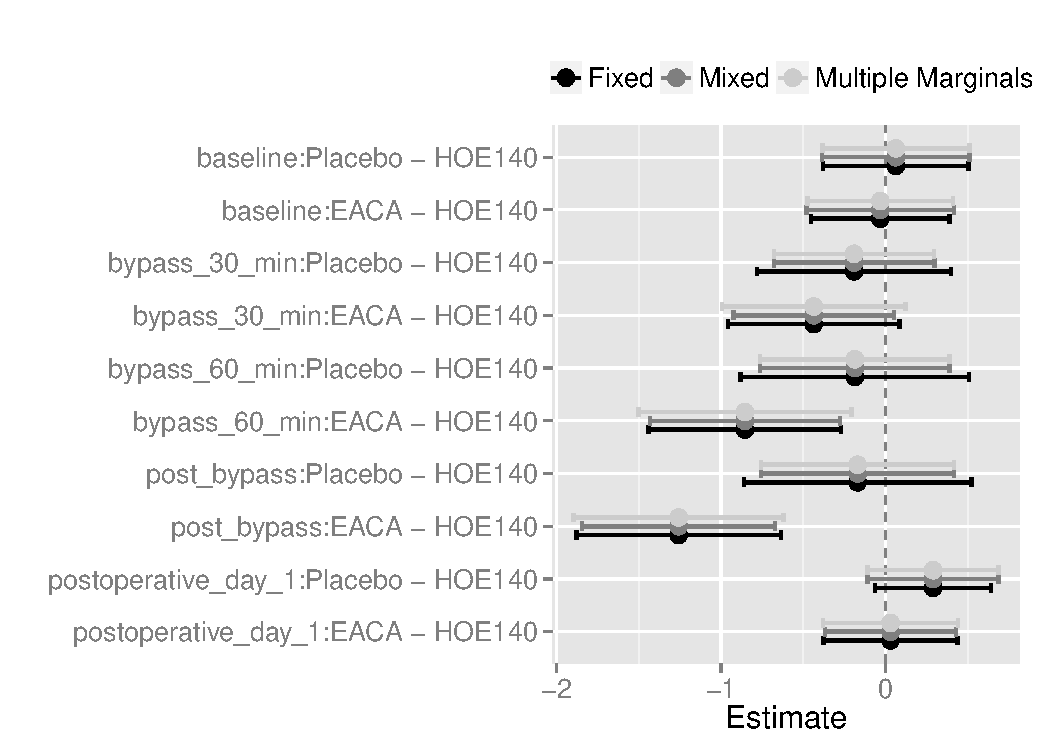
\includegraphics[width=\maxwidth]{figure/PLOTSCI} 

\end{knitrout}


\clearpage

%%%%%%%%%%%%%%%%%%%%%%%%%%%%%%%%%%%%%%%%%%%%%%%%%%%%%%%%%%%%%%%%%%%%%%%%%%%%%%%%%%%%%%%%%%%%%%%%%%%%%%%%%%%%%%%%%%%%%%%%%%%%%%%%%%
%%%%%%%%%%%%%%%%%%%%%%%%%%%%%%%%%%%%%%%%%%%%%%%%%%%%%%%%%%%%%%%%%%%%%%%%%%%%%%%%%%%%%%%%%%%%%%%%%%%%%%%%%%%%%%%%%%%%%%%%%%%%%%%%%%
%%%%%%%%%%%%%%%%%%%%%%%%%%%%%%%%%%%%%%%%%%%%%%%%%%%%%%%%%%%%%%%%%%%%%%%%%%%%%%%%%%%%%%%%%%%%%%%%%%%%%%%%%%%%%%%%%%%%%%%%%%%%%%%%%%

\nocite{*}

\bibliographystyle{abbrvnat}
\bibliography{vign}

\end{document}
